\documentclass[10pt]{article}

\usepackage{amsmath} \allowdisplaybreaks
\usepackage{amssymb}
\usepackage[hyphens]{url}

\usepackage[T1]{fontenc}
\usepackage[polish,english]{babel}
\usepackage[utf8]{inputenc}
\usepackage{lmodern}

\usepackage[en]{csagh}
\usepackage{graphics}
\usepackage{graphicx}

\makeatletter

\begin{document}

\begin{opening}

\tytulPL{PLATFORMA DO AKTUALIZACJI OPROGRAMOWANIA NA URZĄDZENIACH MOBILNYCH OPARTA NA TECHNOLOGII ERLANG}

\titleEN{ERLANG-BASED SOFTWARE UPDATE PLATFORM FOR MOBILE DEVICES}

\author{Małgorzata Wielgus\affiliation
            {AGH University of Science and Technology,
             Kraków, Poland,
             \texttt{malgorza@student.agh.edu.pl}},
        Przemysław Dąbek\affiliation
           {AGH University of Science and Technology,
             Kraków, Poland,
             \texttt{przemyslaw.dabek@gmail.com}},
        Roman Janusz\affiliation
           {AGH University of Science and Technology,
             Kraków, Poland,
             \texttt{roman@student.agh.edu.pl}},
        \\Tomasz Kowal\affiliation
           {AGH University of Science and Technology,
             Kraków, Poland,
             \texttt{tomekowal@gmail.com}},
        Wojciech Turek\affiliation
            {AGH University of Science and Technology,
             Kraków, Poland,
             \texttt{wojciech.turek@agh.edu.pl}}}

%\date{Kraków, 15 wrzesśnia 2004}

\begin{streszczenie}
To pisze się na samym końcu

\slowakluczowe {Erlang, aktualizacja oprogramowania, urządzenia przenośne}
\end{streszczenie}

\begin{abstract}
To be written at the very end

\keywords{Erlang, software updates, mobile devices}
\end{abstract}

\end{opening}


% SECTIONS

\section{Introduction}

\begin{itemize}
	Fast development of mobile devices creates new domain of applications for large systems composed of many devices communicating over the internet. Those devices can be far from each other, what makes direct access difficult. Our system was designed to simplify software updates on groups of such devices.

	There are many areas of applications including:
    \begin{itemize}
    \item Monitoring - with our system we can perform software updates on cameras in the building. Especially if they are equiped with software for face recognition.
    \item Management of geographically spread devices.
    \item Security - updates on sensors used in cars or alarms in homes.
    \item Robotics - autonomic robots used in factories and in industry.
    \end{itemize}
	 The need: management and software updates, use cases
    General usecase of our system is to perform software updates on multiple devices over unreliable network. There is a need of such updates because of growing amount of remote devices such as sensors, mobile phones or network infrastructure devices. 
	\item Existing solutions include Mobile Devices Management systems created by Nokia, Motorola, Oracle and by Open Mobile Alliance. %cytaty 
	\item ``The tool described in this paper is a response for all the needs world has... ``
\end{itemize}



\section{Requirements and assumptions}

\begin{itemize}
\item Network infrastructure assumptions
\begin{itemize}
\item Possibility of NAT
\item Slow and unreliable connections
\end{itemize}
\item Need for scalability (up to about 10000 devices)
\item Simple, intuitive interface
\item Managing groups of devices, batch updates
\end{itemize}

\section{Erlang Technology Overview}

\begin{itemize}
	\item Usability of Erlang Technology in distributed systems -- general features, advantages
	\item General description of Erlang OTP
	\item Application and releases in Erlang
	\item Updating Erlang applications 
	\item Problems with using the method: 1. system admins are used to apt; 2. management of many devices is hard
\end{itemize}

\section{Packaging of Erlang software}

\subsection{The idea and motivation}

By `packaging of Erlang software`, we mean a way of putting the contents of Erlang node
into packages like {\tt .deb}. These would be easy to install, upgrade and remove with standard
package manager commands. We also want to maintain ability to perform upgrades without
stopping the node (hot code swapping).

There are a few reasons why we decided to implement this:

\begin{itemize}
\item Easy installation and deinstallation of Erlang node on the target system using a single command.
\item Reduction of amount of data downloaded during the upgrade (only the actually changed packages
are fetched by the package manager).
\item Overall better integration with the target system.
\end{itemize}

\subsection{Implementation details}

We decided to create tools to build debian packages {\tt .deb} that would span the contents
of the Erlang node and create a set of packages ready to be pushed to a repository and easily installed
on the target device. This also required general implementation of debian maintainer scripts
included into these packages. These scripts are responsible for management of the node
during installation. Most importantly, they contain the code that performs the upgrade process.

\subsubsection{Decomposition of the Erlang node into debian package set}

The Erlang node is decomposed into a set of debian packages in the following way:
\begin{itemize}
\item Base package contains ERTS and its version is equal to the ERTS version. This package is
architecture-dependent. It has no dependencies.
\item Each Erlang application gets its own package. Its version is equal to the application version.
Package dependencies reflect the list of dependent applications in the {\tt .app} file.
\item Erlang release files are packaged into the final, main package. This package is dependent on the base
package and packages for all applications contained in the release. These dependencies are strict in terms
of version of dependent packages - the release requires a concrete version of every application as well as the ERTS.
\end{itemize}

The only package that should be explicitly maintained by system administrator is the main package containing the release files.
This package, thanks to its well-defined dependencies, represents the whole Erlang node and its installation will cause
the whole node to be deployed on the device.

The point of splitting up the node into several packages related through dependencies was to reduce the amount
of data downloaded during the upgrade process. It is a very common situation when we want to upgrade e.g. only
one Erlang application. Standard Erlang features do not allow us to independently upgrade each application - we must
always create a new version of the whole release and upgrade the release itself. Without proper decomposition of the contents
of the release, this would force us to download a big package containing every application, even though most of them did not change.

Usage of package manager solves this problem. When the node is decomposed into several packages, upgrade of the main package
forces the package manager to download only these application packages whose version changed. This is all thanks to automatic
dependency resolution provided by the package manager.

\subsubsection{Upgrade of the release - maintainer scripts' job}

There are a few maintainer scripts (see \cite{maintainerscripts}) in all the packages spanning the Erlang node.
They are responsible for starting the node when it gets installed, stopping it when it gets
removed and, most importantly, performing the release upgrade process when the main package is being
upgraded by the package manager.

The script performing the release upgrade checks whether the node is running, using tools available in the node {\tt bin} directory.
When the node is running, the script remotely calls appropriate Erlang code on the running node, causing it to switch to the higher
version of the release (standard Erlang release upgrade using the {\tt release\_handler}, without stopping the node).
Hot upgrade may fail or the node may have been down from the beginning. If so, a manual replacement of the old version of the release with the new version is performed (manual replacement of some files) and the node is started.

\subsection{Results and effects}

We were able to implement all crucial features regarding integration of package manager
with Software Update Platform.

From the point of view of an erlang developer maintaining the software being upgraded, the main
feature implemented are a few helpful scripts. They allow easy generation of debian packages from
an Erlang release generated with {\tt rebar} (you can read more about development model in \ref{devmodel}).
There is also a script for easy generation of the {\tt relup} file.

From the point of view of a target system administrator, the main advantage of package manager
is mentioned earlier easy way to install, upgrade and remove the Erlang node. The only configuration
needed at the target system is addition of debian repository in the {\tt apt} configuration file.

From the point of view of an user of the Software Update Platform, main feature implemented is
a built-in debian packages repository along with an UI to manage its contents.

We were also successful in obtaining desired non-functional features of the system regarding its use
of package manager. This includes smaller downloads from the server to the target devices and ability
to use hot-code swapping by the package manager during upgrade process.

\subsection{Problems and limitations}

Although the integration of package was successful, due to a significant mismatch between
how package manager works and how standard Erlang upgrade tools work, some workarounds
were required.

The main problem that we encountered was an issue that we had to resolve when trying
to preserve ability to perform hot-upgrade without stopping the system. Erlang upgrade tools
require that at the point of a release upgrade, the whole old version of the release and the whole new
version of the release are present in the filesystem. When the release is split into several packages, 
it is impossible to find a moment where this requirement is met. It is also impossible to
influence the way package manager works to force it to behave as we wanted.

Because of that, we had to introduce a workaround. Erlang application and Erlang release packages
do not contain their contents directly. Instead, an intermediate {\tt tar.gz} archive is created that
contains actual contents of the package. This archive is then put into the {\tt .deb} file directly.
Like this, we have full control over when the files from the intermediate package are unpacked and
removed. The intermendiate archive is unpacked from the {\tt .deb} file by the package manager directly, while
the actual files are unpacked by the maintainer scripts.

One downside of this approach is that we also had to manually remove application and release files using maintainer scripts.
Another one is that when an application is removed from the release, we have to manually remove the package containing that
application. This cannot be done from the maintainer scripts as it is probably a bad idea to invoke package manager from scripts
invoked by the package manager.

\section{Software Update Platform}

Software Update Platform is responsible for performing updates on multiple devices and monitoring
installed applications. Developers prepare \emph{.deb} packages with applications and add them to
repository. When connection with device is established and information about update is written in
database, platform will perform software update on that device.


\subsection{Architecture}

Software Update Platform consists of two main parts (see \textbf{fig.}~\ref{fig:architecture}):
\begin{itemize}
  \item client application installed on mobile device,
  \item server.
\end{itemize}

\begin{figure}[htbp]
  \centering
    \scalebox{0.9}{%
      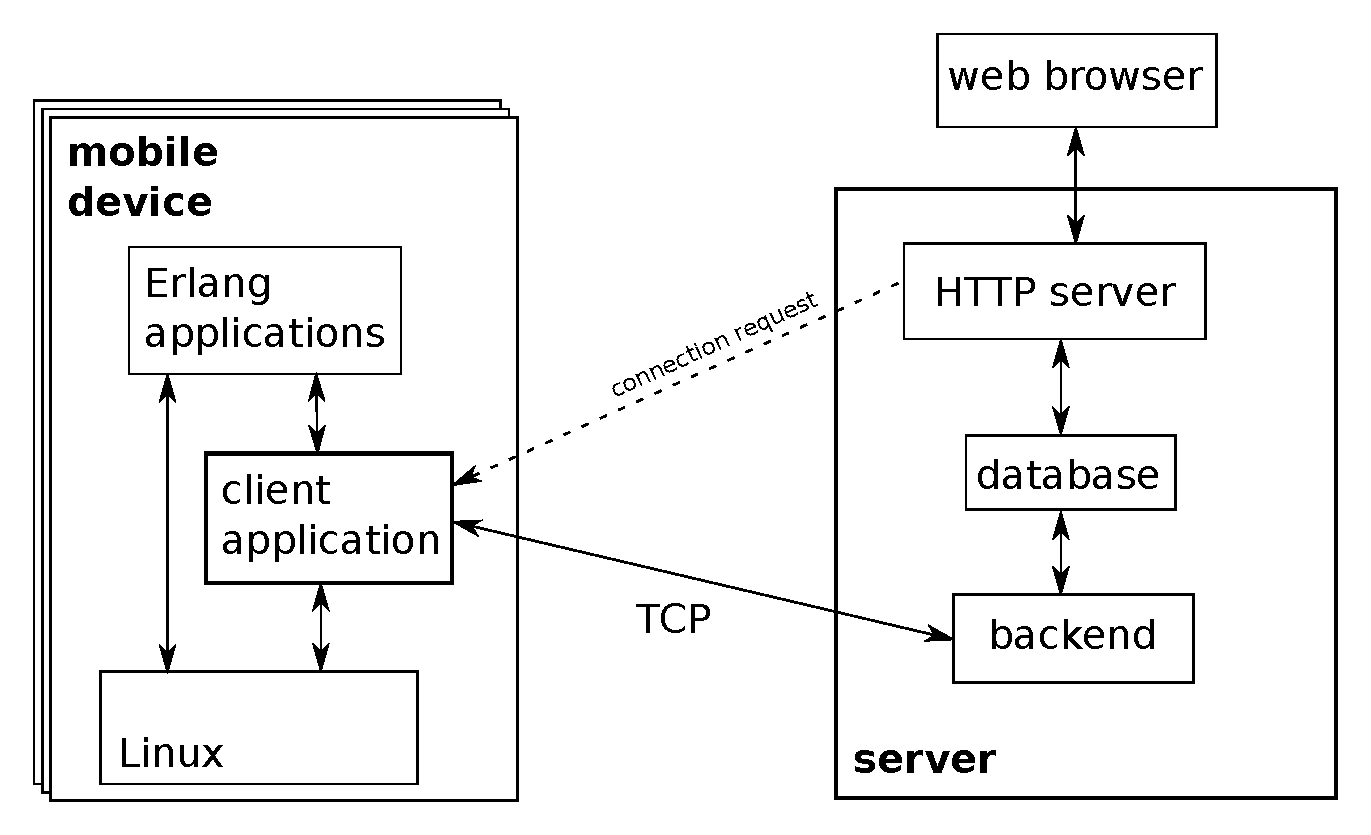
\includegraphics[width=\textwidth]{graphics/architecture.pdf}
    }
    \caption{General architecture of the Software Update Platform}
    \label{fig:architecture}
\end{figure}

\subsubsection*{Client application}

We assume that client application is running on Erlang VM installed on some Linux distribution and
\emph{apt} is available. Client application connects with server and perform given operations.


\subsubsection*{Server}

Server consists of 3 components:
\begin{itemize}
  \item HTTP server
  \item database
  \item backend
\end{itemize}


\subsubsection*{HTTP server}

Mochiweb -- HTTP server manages user interaction through web interface (serves content, performs user requests)
and works as repository for \emph{.deb} packages.

\subsubsection*{Database}

Mnesia database stores information about:
\begin{itemize}
  \item device and installed applications on it,
  \item jobs (e.g.\ update) for device.
\end{itemize}

\noindent Database is connector beetwen web interface and backend. It stores user requests -- jobs to perform
on device.


\subsubsection*{Backend}

Backend is the core of platform. It is Erlang application responsible for whole automatic device
management. Every new device in platform connects with backend and information about this device is stored in database.
From now on backend can monitor state of that device and performs operations on it.

\subsubsection{Device-server session}

\begin{figure}[htbp]
  \centering
    \scalebox{0.9}{%
      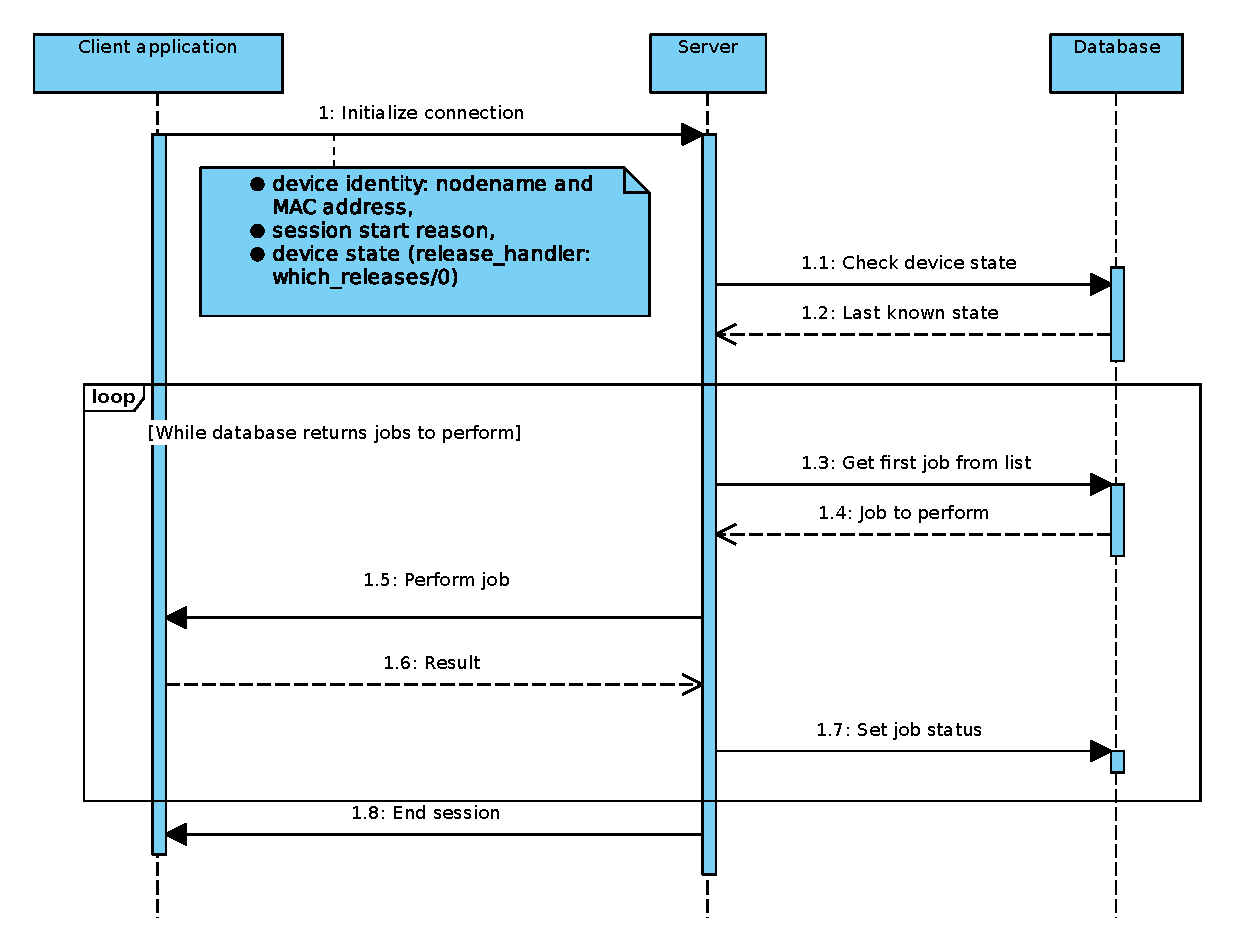
\includegraphics[width=\textwidth]{graphics/session.pdf}
    }
    \caption{Device-server session communication diagram}
    \label{fig:session}
\end{figure}

\noindent Session between device and server (see \textbf{fig.}~\ref{fig:session} above) consists of following steps:

\begin{enumerate}
  \item Device initializes connection which carries following data:
    \begin{itemize}
      \item device identity: nodename and MAC address,
      \item session start reason,
      \item device states.
  \end{itemize}
  These pieces of information are used to unambiguously identify the device.
  \item After connection is established, server checks device state in database.
  If there are any enqueued jobs, they are sent to device.
  \item The device returns result of performed job. This status is written to database.
\end{enumerate}

\subsubsection{On-device upgrade logic}
After receiving a task a device starts the update process. Updating software consists of two jobs:
\begin{itemize}
  \item upgrade
  \item check release
\end{itemize}

Upgrade immediately returns with status \verb|ok|. It stops periodic connection requests, closes session and uses \emph{apt} to perform upgrade. It waits for \emph{apt} to finish and checks its result. Then it restores periodic connection requests.

Check release reads value returned from \emph{apt} and notifies server about changes in next session.

Update process doesn't interrupt running processes and services on device. 

\subsection{Functionality}

\subsubsection{General description of the Web interface}

Web interface provides simple way to manage groups of devices (see \textbf{fig.}~\ref{fig:gui}). User can:
\begin{itemize}
  \item check last known state of device: IP, version of release, installed application
  \item assign device to one or more categories
  \item schedule jobs for device
\end{itemize}

\begin{figure}[htbp]
  \centering
    \scalebox{0.9}{%
      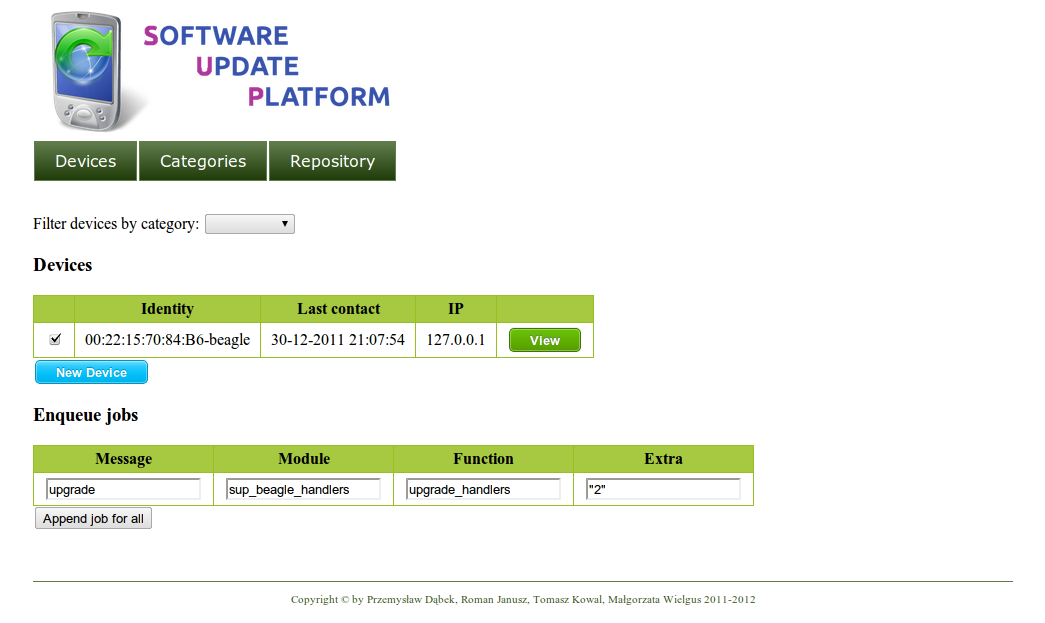
\includegraphics[width=\textwidth]{graphics/devices.png}
    }
    \caption{Web interface -- managing devices by category}
    \label{fig:gui}
\end{figure}

There is also special page for repository where user can upload previously prepared packages.

\subsubsection{Development model for application, debian packaging utilities}
\label{devmodel}

Software Update Platform proposes a model and provides some tools for development of Erlang software installed
on the target systems. The main assumption is that the developer uses a tool called \texttt{rebar} for managing Erlang software (see \cite{rebar} for more information).
\texttt{rebar} is a script providing functionality for Erlang similar to what \texttt{maven} provides for Java development.
This includes automatic generation of stubs for Erlang applications, build, \texttt{.appup} file
generation, creation of complete, self-contained Erlang nodes (with a runtime), documentation etc.
Generated Erlang nodes are used as a basis for \texttt{.deb} packages generation. This is implemented by a set of
scripts provided by the Software Update Platform itself.


\section{Conclusions and Further Work}

To be written at the very end 



% BIBLIOGRAPHY
\begin{thebibliography}{99}

\bibitem{nokia}
\emph{Nokia Device management} \\
\url{http://europe.nokia.com/find-products/nokia-for-business/device-management}

\bibitem{motorola}
\emph{Motorola Mobility Services Platform (MSP)} \\
\url{http://www.motorola.com/Business/US-EN/Business+Product+and+Services/Software+and+Applications/Mobility+Software/Mobile+Device+Management+Software/Mobility+Services+Platform_US-EN}

\bibitem{oracle}
\emph{Oracle Database Mobile Server 11g} \\
\url{http://www.oracle.com/technetwork/database/database-mobile-server/overview/index.html}

\bibitem{oma}
\emph{Open Mobile Alliance} \\
\url{http://www.openmobilealliance.org/}

\bibitem{otp}
\emph{OTP Design Principles} \\
\url{http://www.erlang.org/doc/design_principles/users_guide.html}

\bibitem{maintainerscripts}
\emph{Debian Policy Manual - Package maintainer scripts and installation procedure} \\
\url{http://www.debian.org/doc/debian-policy/ch-maintainerscripts.html}

\bibitem{rebar}
\emph{Rebar: Erlang Build Tool} \\
\url{https://github.com/basho/rebar/wiki}

\end{thebibliography}

\end{document}
